\subsection{Bicycle model of the car}

\begin{figure}
\centering
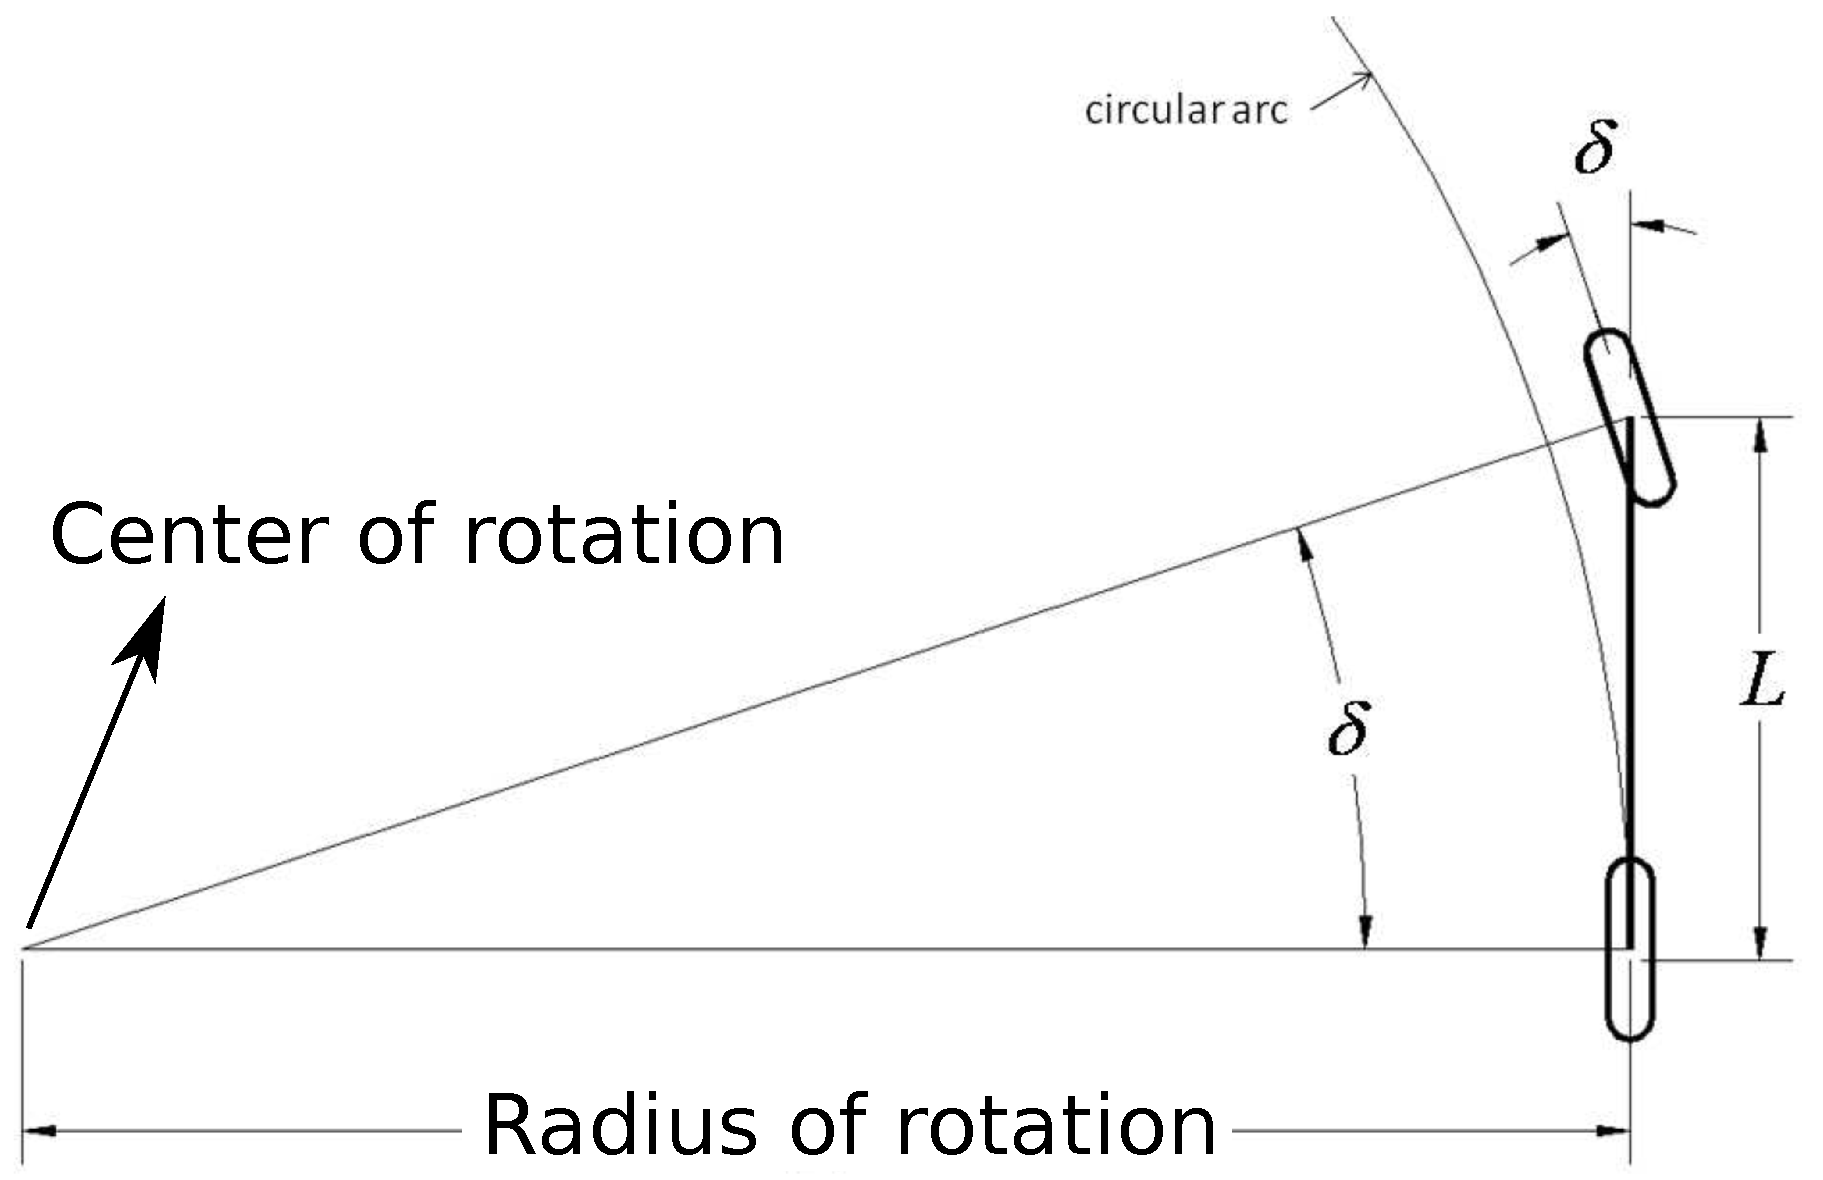
\includegraphics[width=85mm]{Figures/BicycleModel.pdf}%
\caption{Bicycle model \cite{Snider.2009}}
\label{fig:bicycle}%
\end{figure}
In this model (Figure~\ref{fig:bicycle}),
the assumption is that no wheel has lateral slippage.
Therefore,
if the steering angle is $\delta > 0$ and the wheelbase is $L$,
then the rear wheel moves on a circle of radius $R$ where
\begin{equation}
R = \frac{L}{tan(\delta)}.
\end{equation}